% Created by tikzDevice version 0.12.3.1 on 2023-05-05 12:23:03
% !TEX encoding = UTF-8 Unicode
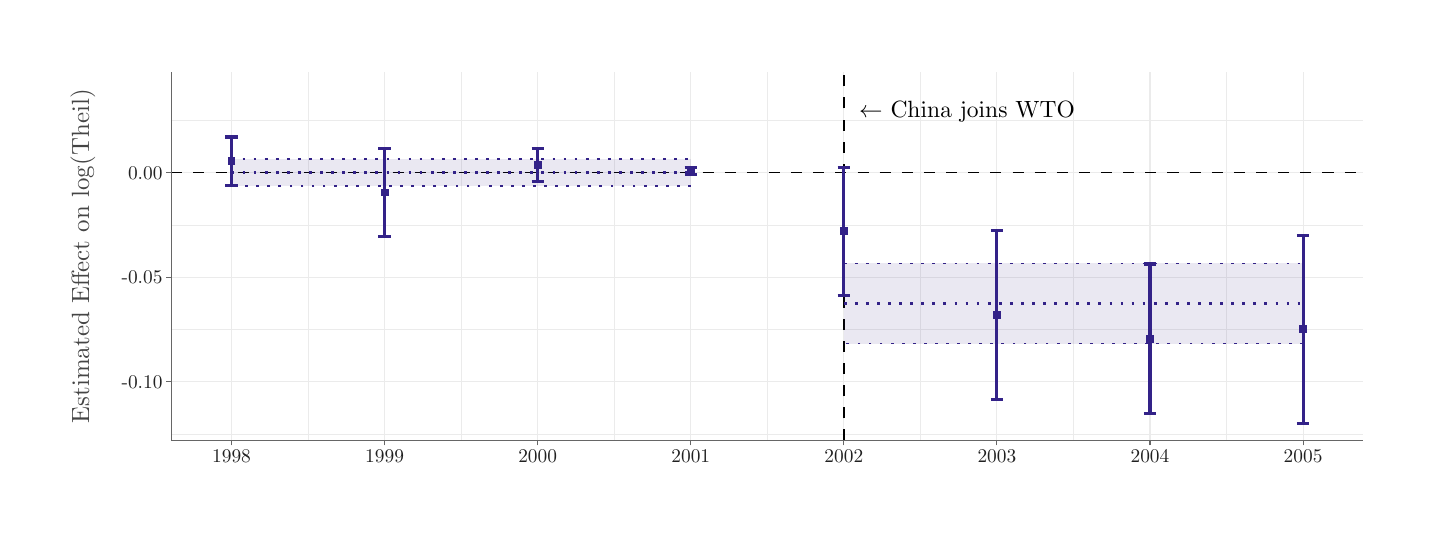
\begin{tikzpicture}[x=1pt,y=1pt]
\definecolor{fillColor}{RGB}{255,255,255}
\path[use as bounding box,fill=fillColor,fill opacity=0.00] (0,0) rectangle (498.66,174.53);
\begin{scope}
\path[clip] (  0.00,  0.00) rectangle (498.66,174.53);
\definecolor{fillColor}{RGB}{255,255,255}

\path[fill=fillColor] (  0.00,  0.00) rectangle (498.66,174.53);
\end{scope}
\begin{scope}
\path[clip] ( 51.87, 25.33) rectangle (482.66,158.53);
\definecolor{fillColor}{RGB}{255,255,255}

\path[fill=fillColor] ( 51.87, 25.33) rectangle (482.66,158.53);
\definecolor{drawColor}{gray}{0.92}

\path[draw=drawColor,line width= 0.2pt,line join=round] ( 51.87, 27.60) --
	(482.66, 27.60);

\path[draw=drawColor,line width= 0.2pt,line join=round] ( 51.87, 65.44) --
	(482.66, 65.44);

\path[draw=drawColor,line width= 0.2pt,line join=round] ( 51.87,103.28) --
	(482.66,103.28);

\path[draw=drawColor,line width= 0.2pt,line join=round] ( 51.87,141.13) --
	(482.66,141.13);

\path[draw=drawColor,line width= 0.2pt,line join=round] (101.32, 25.33) --
	(101.32,158.53);

\path[draw=drawColor,line width= 0.2pt,line join=round] (156.63, 25.33) --
	(156.63,158.53);

\path[draw=drawColor,line width= 0.2pt,line join=round] (211.95, 25.33) --
	(211.95,158.53);

\path[draw=drawColor,line width= 0.2pt,line join=round] (267.27, 25.33) --
	(267.27,158.53);

\path[draw=drawColor,line width= 0.2pt,line join=round] (322.58, 25.33) --
	(322.58,158.53);

\path[draw=drawColor,line width= 0.2pt,line join=round] (377.90, 25.33) --
	(377.90,158.53);

\path[draw=drawColor,line width= 0.2pt,line join=round] (433.21, 25.33) --
	(433.21,158.53);

\path[draw=drawColor,line width= 0.4pt,line join=round] ( 51.87, 46.52) --
	(482.66, 46.52);

\path[draw=drawColor,line width= 0.4pt,line join=round] ( 51.87, 84.36) --
	(482.66, 84.36);

\path[draw=drawColor,line width= 0.4pt,line join=round] ( 51.87,122.20) --
	(482.66,122.20);

\path[draw=drawColor,line width= 0.4pt,line join=round] ( 73.66, 25.33) --
	( 73.66,158.53);

\path[draw=drawColor,line width= 0.4pt,line join=round] (128.98, 25.33) --
	(128.98,158.53);

\path[draw=drawColor,line width= 0.4pt,line join=round] (184.29, 25.33) --
	(184.29,158.53);

\path[draw=drawColor,line width= 0.4pt,line join=round] (239.61, 25.33) --
	(239.61,158.53);

\path[draw=drawColor,line width= 0.4pt,line join=round] (294.92, 25.33) --
	(294.92,158.53);

\path[draw=drawColor,line width= 0.4pt,line join=round] (350.24, 25.33) --
	(350.24,158.53);

\path[draw=drawColor,line width= 0.4pt,line join=round] (405.55, 25.33) --
	(405.55,158.53);

\path[draw=drawColor,line width= 0.4pt,line join=round] (460.87, 25.33) --
	(460.87,158.53);
\definecolor{drawColor}{RGB}{0,0,0}

\path[draw=drawColor,line width= 0.6pt,dash pattern=on 4pt off 4pt ,line join=round] ( 51.87,122.20) -- (482.66,122.20);

\path[draw=drawColor,line width= 0.6pt,dash pattern=on 4pt off 4pt ,line join=round] (294.92, 25.33) -- (294.92,158.53);

\node[text=drawColor,anchor=base west,inner sep=0pt, outer sep=0pt, scale=  0.85] at (300.45,141.97) {$\leftarrow$ China joins WTO};
\definecolor{drawColor}{RGB}{51,34,136}

\path[draw=drawColor,line width= 1.1pt,line join=round] ( 71.45,135.02) --
	( 75.87,135.02);

\path[draw=drawColor,line width= 1.1pt,line join=round] ( 73.66,135.02) --
	( 73.66,117.40);

\path[draw=drawColor,line width= 1.1pt,line join=round] ( 71.45,117.40) --
	( 75.87,117.40);

\path[draw=drawColor,line width= 1.1pt,line join=round] (126.76,130.88) --
	(131.19,130.88);

\path[draw=drawColor,line width= 1.1pt,line join=round] (128.98,130.88) --
	(128.98, 99.03);

\path[draw=drawColor,line width= 1.1pt,line join=round] (126.76, 99.03) --
	(131.19, 99.03);

\path[draw=drawColor,line width= 1.1pt,line join=round] (182.08,130.81) --
	(186.51,130.81);

\path[draw=drawColor,line width= 1.1pt,line join=round] (184.29,130.81) --
	(184.29,118.98);

\path[draw=drawColor,line width= 1.1pt,line join=round] (182.08,118.98) --
	(186.51,118.98);

\path[draw=drawColor,line width= 1.1pt,line join=round] (237.40,123.95) --
	(241.82,123.95);

\path[draw=drawColor,line width= 1.1pt,line join=round] (239.61,123.95) --
	(239.61,121.55);

\path[draw=drawColor,line width= 1.1pt,line join=round] (237.40,121.55) --
	(241.82,121.55);

\path[draw=drawColor,line width= 1.1pt,line join=round] (292.71,124.06) --
	(297.14,124.06);

\path[draw=drawColor,line width= 1.1pt,line join=round] (294.92,124.06) --
	(294.92, 77.87);

\path[draw=drawColor,line width= 1.1pt,line join=round] (292.71, 77.87) --
	(297.14, 77.87);

\path[draw=drawColor,line width= 1.1pt,line join=round] (348.03,101.32) --
	(352.45,101.32);

\path[draw=drawColor,line width= 1.1pt,line join=round] (350.24,101.32) --
	(350.24, 40.20);

\path[draw=drawColor,line width= 1.1pt,line join=round] (348.03, 40.20) --
	(352.45, 40.20);

\path[draw=drawColor,line width= 1.1pt,line join=round] (403.34, 89.13) --
	(407.77, 89.13);

\path[draw=drawColor,line width= 1.1pt,line join=round] (405.55, 89.13) --
	(405.55, 35.14);

\path[draw=drawColor,line width= 1.1pt,line join=round] (403.34, 35.14) --
	(407.77, 35.14);

\path[draw=drawColor,line width= 1.1pt,line join=round] (458.66, 99.53) --
	(463.08, 99.53);

\path[draw=drawColor,line width= 1.1pt,line join=round] (460.87, 99.53) --
	(460.87, 31.57);

\path[draw=drawColor,line width= 1.1pt,line join=round] (458.66, 31.57) --
	(463.08, 31.57);
\definecolor{fillColor}{RGB}{51,34,136}

\path[fill=fillColor] ( 72.24,124.79) --
	( 75.09,124.79) --
	( 75.09,127.64) --
	( 72.24,127.64) --
	cycle;

\path[fill=fillColor] (127.55,113.53) --
	(130.40,113.53) --
	(130.40,116.39) --
	(127.55,116.39) --
	cycle;

\path[fill=fillColor] (182.87,123.47) --
	(185.72,123.47) --
	(185.72,126.32) --
	(182.87,126.32) --
	cycle;

\path[fill=fillColor] (238.18,121.32) --
	(241.03,121.32) --
	(241.03,124.18) --
	(238.18,124.18) --
	cycle;

\path[fill=fillColor] (293.50, 99.54) --
	(296.35, 99.54) --
	(296.35,102.40) --
	(293.50,102.40) --
	cycle;

\path[fill=fillColor] (348.81, 69.33) --
	(351.66, 69.33) --
	(351.66, 72.19) --
	(348.81, 72.19) --
	cycle;

\path[fill=fillColor] (404.13, 60.70) --
	(406.98, 60.70) --
	(406.98, 63.56) --
	(404.13, 63.56) --
	cycle;

\path[fill=fillColor] (459.44, 64.12) --
	(462.30, 64.12) --
	(462.30, 66.97) --
	(459.44, 66.97) --
	cycle;
\definecolor{fillColor}{RGB}{51,34,136}

\path[fill=fillColor,fill opacity=0.10] (294.92, 89.36) --
	(460.87, 89.36) --
	(460.87, 60.35) --
	(294.92, 60.35) --
	cycle;

\path[draw=drawColor,line width= 0.6pt,dash pattern=on 1pt off 3pt ,line join=round] (294.92, 89.36) --
	(460.87, 89.36);

\path[draw=drawColor,line width= 0.6pt,dash pattern=on 1pt off 3pt ,line join=round] (460.87, 60.35) --
	(294.92, 60.35);

\path[fill=fillColor,fill opacity=0.10] ( 73.66,127.00) --
	(239.61,127.00) --
	(239.61,117.41) --
	( 73.66,117.41) --
	cycle;

\path[draw=drawColor,line width= 0.6pt,dash pattern=on 1pt off 3pt ,line join=round] ( 73.66,127.00) --
	(239.61,127.00);

\path[draw=drawColor,line width= 0.6pt,dash pattern=on 1pt off 3pt ,line join=round] (239.61,117.41) --
	( 73.66,117.41);

\path[draw=drawColor,line width= 1.1pt,dash pattern=on 1pt off 3pt ,line join=round] (294.92, 74.85) --
	(460.87, 74.85);

\path[draw=drawColor,line width= 1.1pt,dash pattern=on 1pt off 3pt ,line join=round] ( 73.66,122.20) --
	(239.61,122.20);
\end{scope}
\begin{scope}
\path[clip] (  0.00,  0.00) rectangle (498.66,174.53);
\definecolor{drawColor}{gray}{0.40}

\path[draw=drawColor,line width= 0.4pt,line join=round] ( 51.87, 25.33) --
	( 51.87,158.53);
\end{scope}
\begin{scope}
\path[clip] (  0.00,  0.00) rectangle (498.66,174.53);
\definecolor{drawColor}{gray}{0.13}

\node[text=drawColor,anchor=base east,inner sep=0pt, outer sep=0pt, scale=  0.70] at ( 48.72, 44.11) {-0.10};

\node[text=drawColor,anchor=base east,inner sep=0pt, outer sep=0pt, scale=  0.70] at ( 48.72, 81.95) {-0.05};

\node[text=drawColor,anchor=base east,inner sep=0pt, outer sep=0pt, scale=  0.70] at ( 48.72,119.79) {0.00};
\end{scope}
\begin{scope}
\path[clip] (  0.00,  0.00) rectangle (498.66,174.53);
\definecolor{drawColor}{gray}{0.40}

\path[draw=drawColor,line width= 0.4pt,line join=round] ( 50.12, 46.52) --
	( 51.87, 46.52);

\path[draw=drawColor,line width= 0.4pt,line join=round] ( 50.12, 84.36) --
	( 51.87, 84.36);

\path[draw=drawColor,line width= 0.4pt,line join=round] ( 50.12,122.20) --
	( 51.87,122.20);
\end{scope}
\begin{scope}
\path[clip] (  0.00,  0.00) rectangle (498.66,174.53);
\definecolor{drawColor}{gray}{0.40}

\path[draw=drawColor,line width= 0.4pt,line join=round] ( 51.87, 25.33) --
	(482.66, 25.33);
\end{scope}
\begin{scope}
\path[clip] (  0.00,  0.00) rectangle (498.66,174.53);
\definecolor{drawColor}{gray}{0.40}

\path[draw=drawColor,line width= 0.4pt,line join=round] ( 73.66, 23.58) --
	( 73.66, 25.33);

\path[draw=drawColor,line width= 0.4pt,line join=round] (128.98, 23.58) --
	(128.98, 25.33);

\path[draw=drawColor,line width= 0.4pt,line join=round] (184.29, 23.58) --
	(184.29, 25.33);

\path[draw=drawColor,line width= 0.4pt,line join=round] (239.61, 23.58) --
	(239.61, 25.33);

\path[draw=drawColor,line width= 0.4pt,line join=round] (294.92, 23.58) --
	(294.92, 25.33);

\path[draw=drawColor,line width= 0.4pt,line join=round] (350.24, 23.58) --
	(350.24, 25.33);

\path[draw=drawColor,line width= 0.4pt,line join=round] (405.55, 23.58) --
	(405.55, 25.33);

\path[draw=drawColor,line width= 0.4pt,line join=round] (460.87, 23.58) --
	(460.87, 25.33);
\end{scope}
\begin{scope}
\path[clip] (  0.00,  0.00) rectangle (498.66,174.53);
\definecolor{drawColor}{gray}{0.13}

\node[text=drawColor,anchor=base,inner sep=0pt, outer sep=0pt, scale=  0.70] at ( 73.66, 17.36) {1998};

\node[text=drawColor,anchor=base,inner sep=0pt, outer sep=0pt, scale=  0.70] at (128.98, 17.36) {1999};

\node[text=drawColor,anchor=base,inner sep=0pt, outer sep=0pt, scale=  0.70] at (184.29, 17.36) {2000};

\node[text=drawColor,anchor=base,inner sep=0pt, outer sep=0pt, scale=  0.70] at (239.61, 17.36) {2001};

\node[text=drawColor,anchor=base,inner sep=0pt, outer sep=0pt, scale=  0.70] at (294.92, 17.36) {2002};

\node[text=drawColor,anchor=base,inner sep=0pt, outer sep=0pt, scale=  0.70] at (350.24, 17.36) {2003};

\node[text=drawColor,anchor=base,inner sep=0pt, outer sep=0pt, scale=  0.70] at (405.55, 17.36) {2004};

\node[text=drawColor,anchor=base,inner sep=0pt, outer sep=0pt, scale=  0.70] at (460.87, 17.36) {2005};
\end{scope}
\begin{scope}
\path[clip] (  0.00,  0.00) rectangle (498.66,174.53);
\definecolor{drawColor}{gray}{0.27}

\node[text=drawColor,rotate= 90.00,anchor=base,inner sep=0pt, outer sep=0pt, scale=  0.90] at ( 22.20, 91.93) {Estimated Effect on $\log($Theil$)$};
\end{scope}
\end{tikzpicture}
